% bare_jrnl_compsoc, texV1.4b, 2015/08/26, Michael Shell
\documentclass[10pt,journal,compsoc]{IEEEtran}

% *** MISC UTILITY PACKAGES ***

\newcommand{\note}[1]{\textcolor{magenta}{#1}} 
\usepackage[nocompress]{cite}
\usepackage[]{footmisc}
\usepackage{hyperref} % autoref
% *** GRAPHICS RELATED PACKAGES ***
\ifCLASSINFOpdf
   \usepackage[pdftex]{graphicx}
  % declare the path(s) where your graphic files are
   \graphicspath{{./figures/}}
  % and their extensions so you won't have to specify these with
  % every instance of \includegraphics
  % \DeclareGraphicsExtensions{.pdf,.jpeg,.png}
\else
  % or other class option (dvipsone, dvipdf, if not using dvips). graphicx
  % will default to the driver specified in the system graphics.cfg if no
  % driver is specified.
   \usepackage[dvips]{graphicx}
  % declare the path(s) where your graphic files are
   \graphicspath{{./figures/}}
  % and their extensions so you won't have to specify these with
  % every instance of \includegraphics
   \DeclareGraphicsExtensions{.eps}
\fi

% latex, and pdflatex in dvi mode, support graphics in encapsulated
% postscript (.eps) format. pdflatex in pdf mode supports graphics
% in .pdf, .jpeg, .png and .mps (metapost) formats. Users should ensure
% that all non-photo figures use a vector format (.eps, .pdf, .mps) and
% not a bitmapped formats (.jpeg, .png). The IEEE frowns on bitmapped formats
% which can result in "jaggedy"/blurry rendering of lines and letters as
% well as large increases in file sizes.

% *** MATH PACKAGES ***
%% with other math-related packages, you may want to disable it.
\usepackage{amsmath, amsthm, amsfonts,amssymb,eulervm,xspace, mathtools}
\usepackage{mathrsfs} % math script fonts
\theoremstyle{definition}
\newtheorem{definition}{Definition}[section]
\theoremstyle{remark}
\newtheorem{example}{Example}[section]
% *** SPECIALIZED LIST PACKAGES ***
\usepackage{xcolor}
\usepackage{algorithmic}
\usepackage[utf8]{inputenc}
\usepackage{subfig} %ieee does not like subfigure
\usepackage{multicol}
\usepackage{tikz}
\usetikzlibrary{cd} % commutative diagrams
\newtheorem{prop}{Proposition} %math?
\usepackage[switch]{lineno}
\usepackage{minted}
\setminted[python]{fontsize=\scriptsize, 
                   linenos,
                   numbersep=8pt,
                   autogobble, 
                   frame=lines,
                   framesep=3mm} 
% *** ALIGNMENT PACKAGES ***
\usepackage{array}
\usepackage{tabulary}
% IEEEtran contains the IEEEeqnarray family of commands

% *** SUBFIGURE PACKAGES ***
\ifCLASSOPTIONcompsoc
  \usepackage[caption=false,font=footnotesize,labelfont=sf,textfont=sf]{subfig}
\else
  \usepackage[caption=false,font=footnotesize]{subfig}
\fi

% *** FLOAT PACKAGES ***
\usepackage{dblfloatfix}

% *** PDF, URL AND HYPERLINK PACKAGES ***
\usepackage{url}

% *** Do not adjust lengths that control margins, column widths, etc. ***
% *** Do not use packages that alter fonts (such as pslatex).         ***
% There should be no need to do such things with IEEEtran.cls V1.6 and later.
% (Unless specifically asked to do so by the journal or conference you plan
% to submit to, of course. )

\usepackage{notation} %notation conventions
% correct bad hyphenation here
\hyphenation{op-tical net-works semi-conduc-tor}


\begin{document}
%
\title{Topological Equivariant Artist Model for Visualization Library Architecture}
% author names and IEEE memberships
\author{Hannah~Aizenman, Thomas~Caswell, and~Michael~Grossberg,~\IEEEmembership{Member,~IEEE,}% <-this % stops a space
\IEEEcompsocitemizethanks{\IEEEcompsocthanksitem H. Aizenman and M. Grossberg are with the department of Computer Science, City College of New York. 
\protect\\
% note need leading \protect in front of \\ to get a newline within \thanks as
% \\ is fragile and will error, could use \hfil\break instead.
E-mail: haizenman@ccny.cuny.edu, mgrossberg@ccny.cuny.edu 
\IEEEcompsocthanksitem Thomas Caswell is with National Synchrotron Light Source II, Brookhaven National Lab 
\protect \\
E-mail: tcaswell@bnl.gov}% <-this % stops an unwanted space
\thanks{Manuscript received X XX, XXXX; revised X XX, XXXX.}
}


% for Computer Society papers, we must declare the abstract and index terms
% PRIOR to the title within the \IEEEtitleabstractindextext IEEEtran
% command as these need to go into the title area created by \maketitle.
% As a general rule, do not put math, special symbols or citations
% in the abstract or keywords.
\IEEEtitleabstractindextext{%
\begin{abstract}
The abstract goes here.
\end{abstract}

% Note that keywords are not normally used for peerreview papers.
\begin{IEEEkeywords}
%Computer Society, IEEE, IEEEtran, journal, \LaTeX, paper, template.
\end{IEEEkeywords}}


% make the title area
\maketitle


\IEEEpeerreviewmaketitle



\IEEEraisesectionheading{\section{Introduction}\label{sec:introduction}}


\IEEEPARstart{T}his paper uses methods from topology and category theory to develop a model of the transformation from data to graphical representation. This model provides a language to specify how data is structured and how this structure is carried through in the visualization, and serves as the basis for a functional approach to implementing visualization library components. Topology allows us to describe the structure of the data and graphics in a generalizable, scalable, and trackable way. Category theory provides a framework for separating the transformations implemented by visualization libraries from the various stages of visualization and therefore can be used to describe the constraints imposed on the library components \cite{wielsManagementEvolvingSpecifications1998,goguenCategoricalManifesto1991}. Well constrained modular components are inherently functional\cite{hughesWhyFunctionalProgramming1989}, and a functional framework yields a library implementation that is likely to be shorter, clearer, and more suited to distributed, concurrent, and on demand tasks\cite{huHowFunctionalProgramming2015}. Using this functional approach, this paper contributes a practical framework for decoupling data processing from visualization generation in a way that allows for modular visualization components that are applicable to a variety of data sets in different formats. \note{is it OK that this is something reviewer 4 wrote}



\section{Related Work}
This work aims to develop a model for describing visualization transformations that can serve as guidance for how to architecture a general purpose visualization library. We define a general purpose visualization library as one that provides non domain specific building block components\cite{wongsuphasawatNavigatingWideWorld2021} for building visualizations, for example functions for converting data to color or encoding data as dots. In this section, we describe how visualization libraries attempt this goal and discuss work that formally describes what properties of data should be preserved in a visualization. We restrict the properties of data that should be preserved to 

\begin{LaTeXdescription}
  \item [continuity] how elements in a dataset are organized, e.g. discrete rows in a table, networked nodes, pixels in an image, points on a line
  \item [equivariance] functions on data that have an equivalent effect on the graphical representation, e.g. rotating a matrix has a matching rotation of the image, translating the points on a line has a matching visual shift in the line plot
\end{LaTeXdescription}

\subsection{Continuity}
\begin{figure}[!h]
  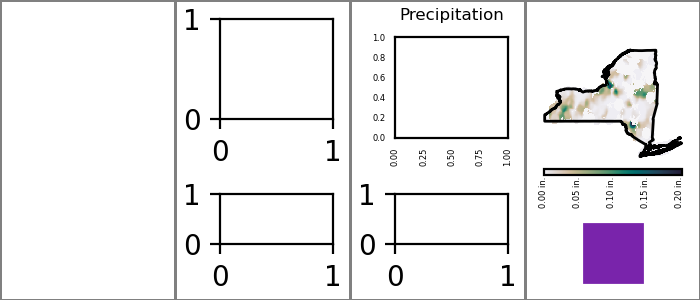
\includegraphics[width=\columnwidth]{k_different_types.png}
  \caption{Continuity is how elements in a data set are connected to each other, which is distinct from how the data is structured. The rows in (a) are discrete, therefore they have discrete continuity as illustrated by the discrete dots. The gaussian in (b) is a 1D continuous function, therefore the continuity of the elements of the gaussian can be represented as a line on an interval (0,1). In (c), every element of the globe is connected to its nearest neighbors, which yields a 2D continuous continuity as illustrated by the square.}
  \label{fig:related-work:continuity}
\end{figure}
Continuity describes elements in a data set are organized; this concept is termed topological properties by Wilkinson\cite{wilkinsonGrammarGraphics2005}. Wilkinson provides the examples of values that are isolated from each other, and therefore discrete, and values lying on a continuum or in a compact region. For example, in \autoref{fig:related-work:continuity}, each station record in the table is independent of the others; therefore, the continuity of the table is discrete. The data provided by the gaussian are points sampled along the curve, therefore the continuity of the points on the line is 1D continuous. Every point on the globe is connected to its 6 nearest cardinal neighboring points (NW, N, NE, E, SE, S, SW, W). We propose that a robust model of continuity provides a way to develop library components that can work on the data in small pieces in a manner where the overall continuity of the data is preserved in the visual transformation. 

\begin{figure}[!h]
  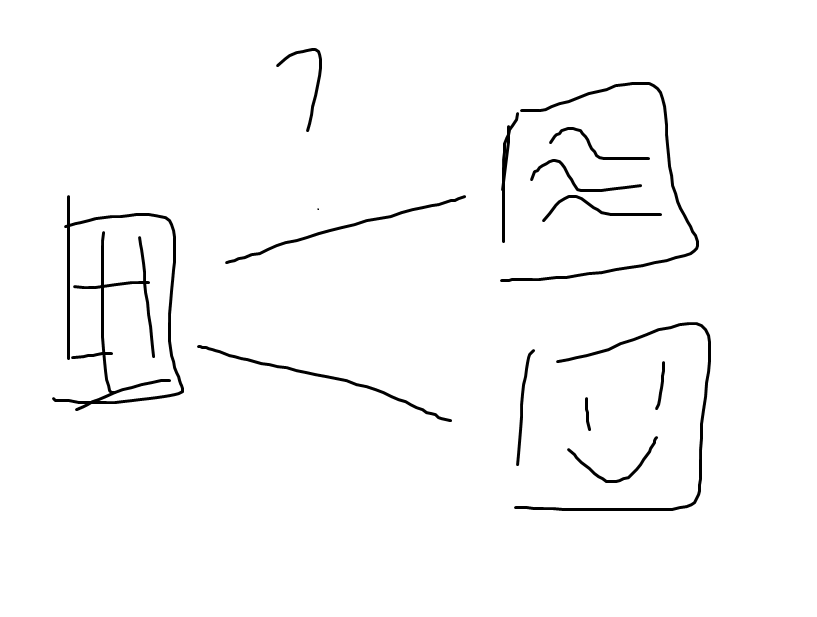
\includegraphics[width=\columnwidth]{whycontinuity.png}
  \caption{Continuity is implicit in choice of visualization rather than explicitly in choice of data container. The line plots in (b) are generated by a 2D table (a). Structurally this table can be identical to the 2D matrix (a) that generates the image in (c).}
  \label{fig:related-work:visual-algorithm}
\end{figure}

 The preservation of continuity can be made explicit, as in the transformation of table to parallel coordinates in Ruchikachorn and Mueller \cite{ruchikachornLearningVisualizationsAnalogy2015}, but is often expressed implicitly in the choice of visual algorithm (visualization type), as explored in taxonomies by Tory and M\"{o}ller \cite{toryRethinkingVisualizationHighlevel2004} and Chi\cite{chiTaxonomyVisualizationTechniques2000}.

For example, in \autoref{fig:related-work:visual-algorithm} the same table can be interpreted as a set of 1D continuous curves when visualized as a collection of line plots or as a 2D surface when visualized as an image.  This means that often there is no way to express data continuity independent of visualization type, meaning most visualization libraries will allow, for example, visualizing discrete data as a line plot or an image. General purpose visualization libraries-such as Matplotlib\cite{hunterMatplotlib2DGraphics2007}, Vtk\cite{hanwellVisualizationToolkitVTK2015,geveciVTK2012}, and D3 \cite{bostockDataDrivenDocuments2011}-carry distinct data models as part of the implementation of each visual algorithm. The lack of unified data model means that each plot in a linked\cite{beckerBrushingScatterplots1987,bujaInteractiveData1991} visualization is treated as independent, as are the transforms converting each field in the data to a visual equivalent.

Domain specific libraries can often guarantee consistency because they have a single model of the data in their software design, as discussed in Heer and Agarwal \cite{HeerSoftware2006}'s survey of visualization software design patterns. For example, the relational database is core to tools influenced by APT, such as Tableau\cite{StoltePolaris2002,hanrahanVizQL2006,MackinlayShowme2007} and the Grammar of Graphics\cite{wilkinsonGrammarGraphics2005} inspired ggplot\cite{wickhamGgplot2ElegantGraphics2016a}, Vega\cite{satyanarayanDeclarativeInteractionDesign2014} and Altair\cite{vanderplasAltairInteractiveStatistical2018}. Images underpin scientific visualization tools such as Napari\cite{nicholas_sofroniew_2021_4533308} and ImageJ\cite{schneiderNIHImageImageJ2012} and the digital humanities oriented ImagePlot\cite{studiesCulturevisImageplot2021} macro; the need to visualize and manipulate graphs has spawned tools like Gephi\cite{bastianGephiOpenSource2009}, Graphviz\cite{ellsonGraphvizOpenSource2002}, and Networkx\cite{HagbergExploringNetwork2008}. 
 
\subsubsection{Fiber Bundles}
\label{sec:related-work:fiber-bundles}
\begin{figure}[h!]
  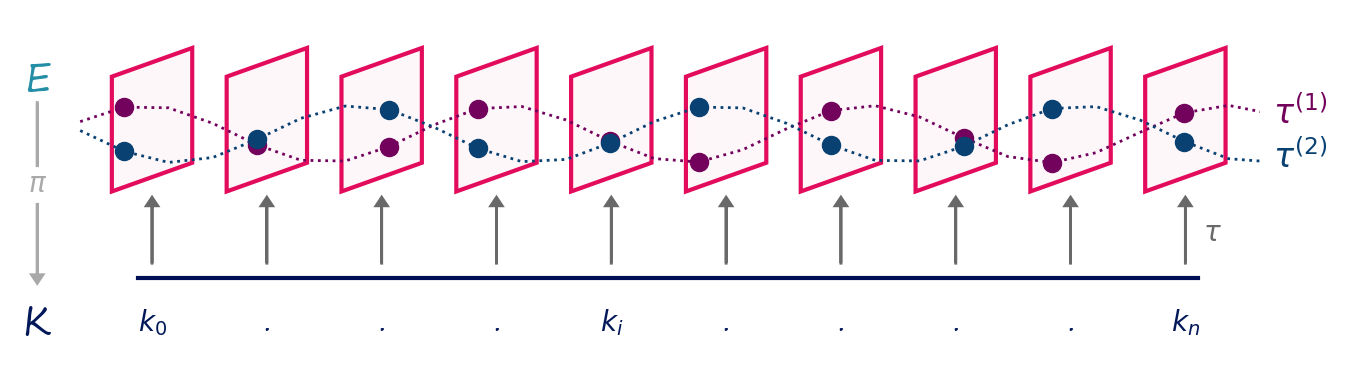
\includegraphics[width=\columnwidth]{fiberbundle.png}
  \caption{A fiber bundle is mathematical construct that allows us to express the relationship between data and continuity. The \textcolor{total}{total} space \dtotal is the topological space in which the data is embedded. The \textcolor{fiber}{fiber} space \dfiber\ is embedded in \dtotal\ and is the set of all possible values that any
  \note{add big rectangle E}}
  \label{fig:related-work:fiber-bundle}
\end{figure}

The model described in this work provides a modol for expressing data sets with different topological properties. 
We obtain this generality by using the mathematical theory of fiber bundles as the basis of our abstraction, as proposed by Butler, Bryson, and Pendley\cite{butlerVisualizationModelBased1989,butlerVectorBundleClassesForm1992}. In this paper, we build on their work that proposes using topological spaces to represent different properties of data.

Specifically,Butler, Bryson, and Pendley suggest that fiber bundles be the basis of an abstract data model. Fiber bundles are a collection of topological spaces. 
\begin{definition}
A topological space $(X, \mathscr{T})$ is a set $X$ with a topology $\mathscr{T}$. Topologies are collections of open sets $U$ such that the empty set and $X$ are in the collection of open sets $\mathscr{T}$, the union of elements in $\mathscr{T}$ \note{finish out this definition}
\end{definition}

Here we present a very brief summary of topics, for more information Hatcher\cite{hatcherAlgebraicTopology2002}, Munkres\cite{munkresElementsAlgebraicTopology1984}, and Spanier \cite{spanier1989algebraic}. 

\begin{LaTeXdescription}
  \item[\textcolor{total}{Total Space} \dtotal]
  \item[\textcolor{fiber}{Fiber Space} \dfiber]
  \item[\textcolor{base}{Base Space} \dbase]  
\end{LaTeXdescription}

with a projection map $\pi:\dtotal\rightarrow\dbase$ that connects every point in \dtotal\ to a point in \dbase. 
\begin{equation}
  \label{eq:fiber_bundle}
  \begin{tikzcd}
      \dfiber \arrow[r, hook] & \dtotal \arrow[r, "\pi"] & \dbase
  \end{tikzcd}
\end{equation}

As indicated by $\hookrightarrow$, the fiber space \dfiber\ is embedded inside the total space \dtotal\. This is illustrated in \autoref{fig:related-work:fiber-bundle}, wherein values lives in the fiber $\dfiber\subseteq\dtotal$. In this example, the fiber \dfiber\ is the cartesian product of two sets $F_{0}\times F_{1}$ where each fiber $F_{i}$ is ....
\begin{equation}
  formal equation of the fiber?
  \label{eq:related-work:fiber}
\end{equation}

While the values are embedded in \dfiber, the continuity of the data is modeled as the base space \dbase, which is the quotient space \cite{QuotientSpaceTopology2020}
\begin{equation}
formal math of the base space as equivalence class for F_[k]
\end{equation}
which means that every point in $\dfiber_{k}$ maps to a point $k \subset K$. 

\begin{equation}
  \begin{tikzcd}
      \dfiber \arrow[r, hook] & \dtotal \arrow[d, "\pi"'] \\
                        & \dbase \arrow[u, "\dsection"', bend right]
  \end{tikzcd}
\end{equation}

Throughout this paper, we denote fiber bundles with the tuple $(\textcolor{total}{total space}, \textcolor{base}{base space}, \pi, \textcolor{fiber}{fiber space})$

\subsection{Equivariance}
\label{sec:related-work:equivariance}
When introducing the retinal variables, Bertin informally specifies that continuity is preserved in the mark and defines equivariance constraints in terms of data and visual variables being selective, associative, ordered, or quantitative\cite{bertinSemiologyGraphicsDiagrams2011a}. In the \textit{A Presentation Tool}(APT) model, Mackinlay embeds the continuity constraint in the choice of visualization type and generalizes the equivariance constraint to preserving a binary operator from one domain to another. The algebraic model of visualization\cite{kindlmannAlgebraicProcessVisualization2014}, proposed by Kindlmann and Scheidegger, restricts equivariance to invertible transformations.

\begin{figure}[!h]
  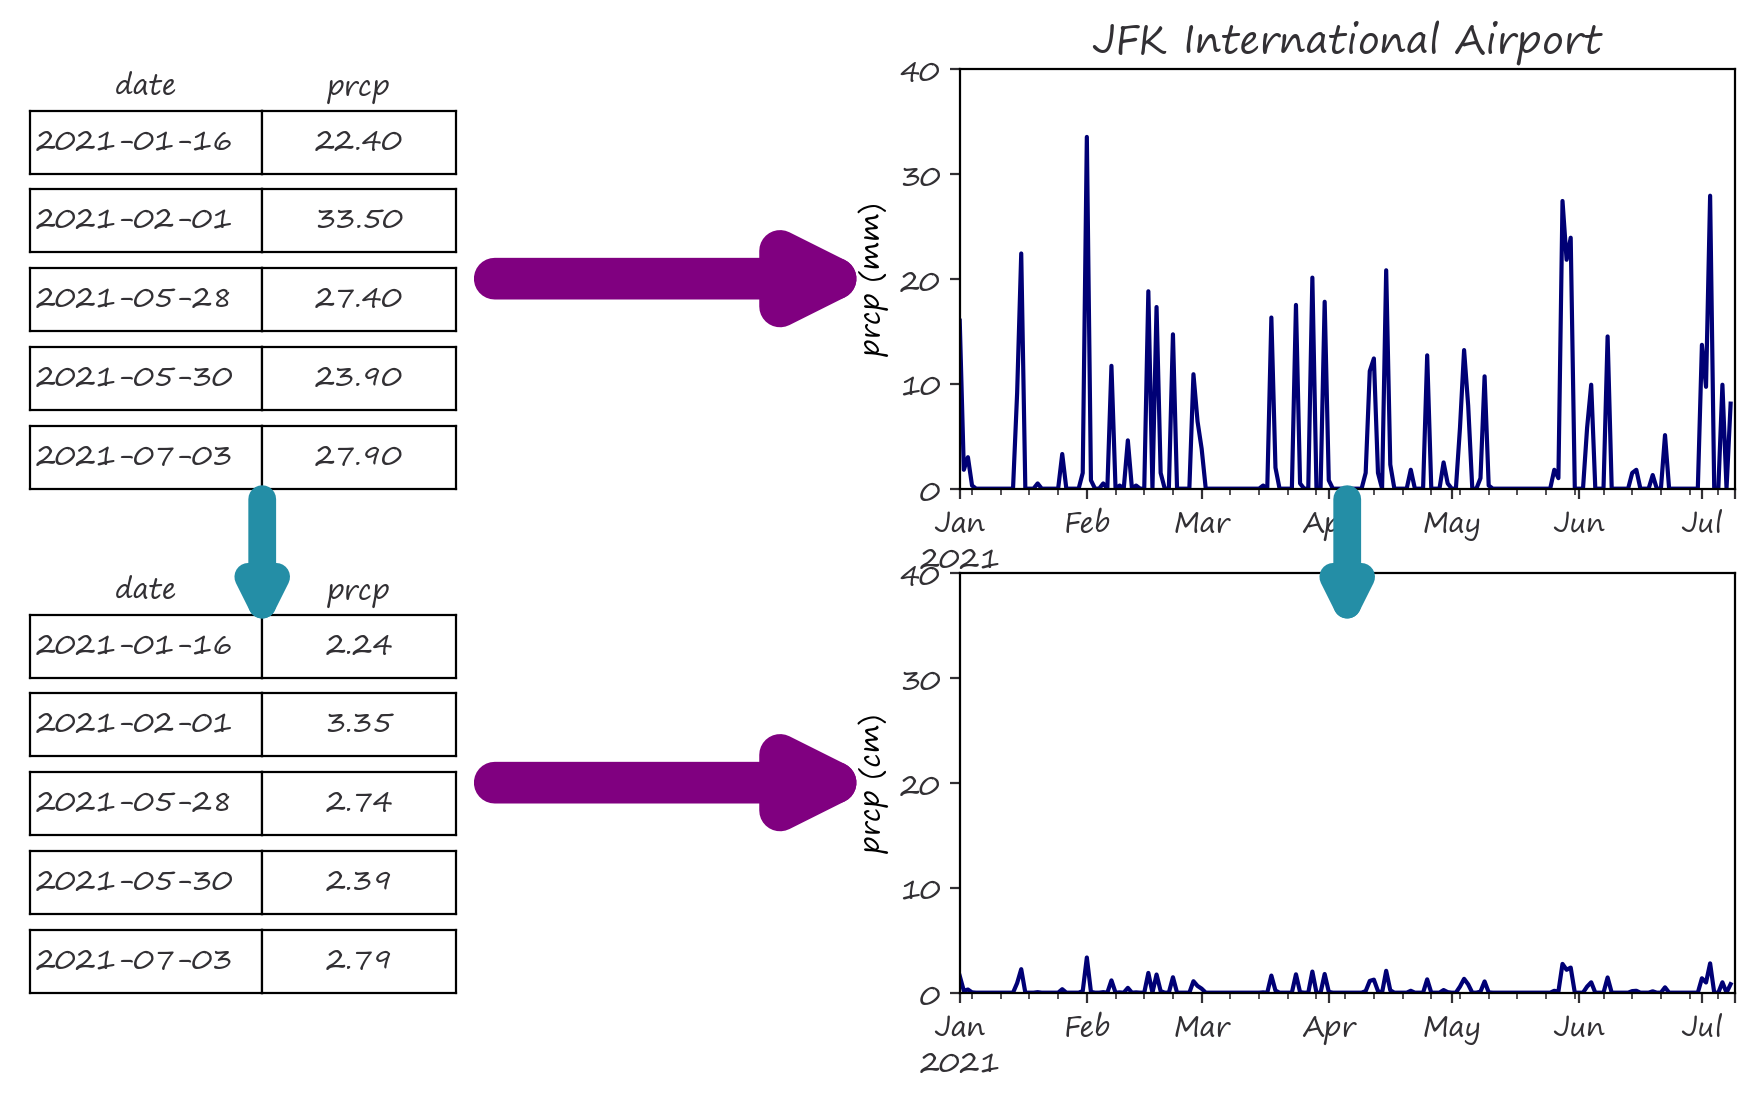
\includegraphics[width=\columnwidth]{equiv.png}
  \caption{Equivariance is that a transformation on the data has a corresponding transformation in the graphical representation. For example, in this figure the data is scaled by a factor 10. Equivalently the line plot is scaled by factor of 10, resulting in a shrunken line plot. Either a transformation on the data side can induce a transformation on the visual side, or a transformation on the visual side indicates that there is also a transformation on the data side. }
\end{figure}

\subsubsection{Category Theory}
\label{sec:related-work:equivariance:category}
In this work, we propose that equivariance constraints can be expressed using category theory. Vickers et. al provide a brief introduction to category theory for visualization practitioners \cite{vickersUnderstandingVisualizationFormal2013}, but their work focuses on data, representation, and evocation, while this paper is aims to provide guidance on how the map from data to representation should be implemented. 

For more information on category theory, see Barr and Wells\cite{barrCategoryTheoryComputing}, Fong and Spivak \cite{fongInvitationAppliedCategory2019}, Riehl\cite{riehlCategoryTheoryContext} and Bradley et. al. \cite{bradleyTopologyCategoricalApproach2020}.

\section{Artist} 
In this section, we use category theory to formally express the implicit assumptions that visualization library components make in transforming data into graphical representations. We propose that the visualization transformation can be modeled as a functor, which we call the \textcolor{artist}{Artist} $\mathcal{\vartist}$\footnote{We call this transformation the artist because the \mintinline{python}{Artist} object in Matplotlib\cite{hunterMatplotlib2DGraphics2007}}. The artist \vartist\ converts data, which we model as the catgory $\mathcal{\dtotal}$ to graphics, which we model as the category $\mathcal{\gtotal}$. We formulate this association as 

\begin{equation}
  \vartist: \mathcal{\dtotal} \rightarrow \mathcal{\gtotal}
  \label{eq:artist:artist}
\end{equation}
In this section we describe the structure of the data and graphic spaces, which we formulate as objects in categories and the morphisms between those objects. We then use these definitions to express the structure that an artist must preserve. Finally, we propose that artists can be composed by manufacturing new artists based on various types of input data. 

\subsection{Categorical Artist}
\label{sec:artist:category}
We define the categories $\mathcal{\dtotal}$ and $\mathcal{\gtotal}$ as sheaves of sections\cite{SheafMathematics2021,spanier1989algebraic}, of fiberbundles, as introduced in \autoref{sec:related-work:fiber-bundles}. Sheaves are mathematical abstractions of how data over different parts of a continuous base space are glued together \cite{ghristElementaryAppliedTopology2014, ghri}, whether the data is distributed, streaming, or in disk; therefore sheaves are a way to express the continuity that the artist preserves. 
We assume that $\mathcal{E}$ is defined in terms of a fixed base and fiber space, for example a class of images or tables with the same schema. The graphic category $\mathcal{\gtotal}$ consists of the set of graphics that an artist \vartist\ is allowed to generate from a given $\mathcal{E}$, which is discussed further in \autoref{sec:artist:construction}.

As introduced in \autoref{sec:related-work:fiber-bundles}, sets of open sets form the basis of topological spaces. We propose that we can express how the elements in our data are connected to each other by modeling the data continuity as a topological space \dbase. We express subsets of the continuity, which can be mapped into subsets of the data, as open sets $U_{i}$ in \dbase. We introduce the category $\mathcal{\dbase}$ to encapsulate the subsets of the continuity and the inclusion maps that glue them together. 

\begin{definition} The category of open sets $\mathcal{\dbase}$ consists of
  \label{def:category:K} 
  \begin{itemize}
    \item \textit{objects} all open sets $U_{i} \in \{U\}$ in the topological space $(\dbase, \mathscr{T})$), including the empty set $\varnothing$ and the maximum set \dbase. 
    \item \textit{morphisms} inclusion maps from a subspace to a larger space $\iota: U_{i} \hookrightarrow U_{j}$, which is equivalent to $U_{i} \subseteq U_{j}$ and  
  \end{itemize} 
\end{definition}

The inclusion maps $\iota$ can be used to piece together the subsets $U_{i}$, particularly individual points $\dbasepoint \in \dbase$. This is how we provide knowledge of continuity to the artist \vartist\ in a way where the artist does not need all the data at once. This is what allows the artist to generate graphics where the subset of data on view is dynamically updated, such as pan and zoom navigation\cite{NekrasovskiEvaluationPanZoom2006} and sliding windows on streaming data\cite{crouchDynamicGraphsSlidingwindow2013,chuTimeSeriesSegmentation1995}. \note{does this actually go down in the composition section?}

Besides expressing continuities, fiber bundles also provide us a way to richly express the structure of the fields in the data. Specifically, we do this by adopting Spivak's formulation of the fiber as a (column name, data domain) simple schema \cite{spivakSIMPLICIALDATABASES,spivakDatabasesAreCategories2010}. Spivak formally maps column names and field types to the set of values associated with the field type, for example $\mathbb{R}$ for a \texttt{float} column named \textit{temperature}. We define $\dfiber$ as  the cartesian cross product of the fibers $\dfiber_c$ for each field, where $c$ is the field name.  

\begin{definition} 
  \label{def:category:F} 
  The category $\mathcal{\dfiber}$ consists of a single object $\dfiber$ and the morphisms between the object and itself $Hom_{\mathcal{\dfiber}}(\dfiber, \dfiber)$, which is the hom-set \cite{maclaneCategoriesWorkingMathematician2013,milewskiCategoryTheoryProgrammers}.
\end{definition}

The object $\texttt{\dfiber}$ can be an object of any category $\mathcal{C}$, allowing $\texttt{\dfiber}$ to encode most data fields. For example, a lists of strings is an instance of an object in \textbf{Set}, networks are an instance of \textbf{Graph}, and images are vector spaces which are a specific type of topological space \textbf{Top}. We note that a one object category is a monoid \cite{nlab:monoid,barrCategoryTheoryComputing}, which is an algebraic structure that lends itself to computer library design because they are an abstraction of function composition \cite{yorgeyMonoidsThemeVariations}. 

The morphisms $Hom_{\mathcal{\dfiber}}(\dfiber, \dfiber)$ are functions from the data to itself, for example the binary operations, group actions, and measurement scales discussed in \autoref{sec:related-work:equivariance}. These functions could also be monoid actions\cite{barrCategoryTheoryComputing}, which provide a way of applying partial order relations to data\cite{fongInvitationAppliedCategory2019}, such as to build multi-ranked indicators\cite{bruggemannRankingPrioritizationMultiindicator2011}

We encode individual datasets in the fiberbundle as sections of the bundle. We follow the convention that $\Gamma(U_i, \dtotal)$ denotes the set of sections $\{\dsection^{j}:U_i \rightarrow \dfiber_{U_{i}}\}_{j\in I}$ of the fiber bundle \dtotal\ over an open set $U_{i}\subseteq \dbase$.  

\begin{definition} The category of sets of sections $\Gamma(U_i,\dtotal)$, where $U_i$ are objects in $\mathcal{\dfiber}$, form a subcatagory of the category of sets \textbf{Set}. The morphisms between objects of this subcategory are restriction maps $\iota: \Gamma(U_j, \dtotal) \rightarrow \Gamma(U_i, \dtotal)$ where $U_{i} \subseteq U_{j}$.
\end{definition}

As mentioned in \autoref{sec:related-work:fiber-bundles}, the fiber space is embedded in the total space $\dfiber \hookrightarrow \dtotal$. The sections $\Gamma(\dbase, \dtotal)$ are called the global sections of $\dtotal$ \cite{SheafMathematics2021,spanier1989algebraic}. Each section is how we represent a unique dataset, where the sets of sections $\Gamma$ is the space of all datasets that have the same data fields in the \dfiber\ and continuity as encoded in\dbase\. For example, Spivak describes tables that have the same schema and discrete index as sections of the same fiber bundle\cite{spivakSIMPLICIALDATABASES}.

\begin{definition} The category $\mathcal{\dtotal}$ consists of 
  \begin{itemize}
    \item\textit{object} the sheaf\cite{SheafMathematics2021,ghristElementaryAppliedTopology2014} $\sheaf_{\mathcal{\dtotal}}: \mathcal{K}^{op} \rightarrow \Gamma(\mathcal{K}, \dtotal)$
    \item \textit{morphisms} arbitrary endomorphic\cite{fongInvitationAppliedCategory2019} bundle maps $\varphi: \dtotal\rightarrow \dtotal$. When the sheaf is restricted to the stalk\cite{StalkSheaf2019} $\mathscr{F}_{k}$ over a point $\dbasepoint\in \dbase$, then allowable morphisms are $\varphi \in Hom_{\mathcal{\dfiber}}(\dfiber,\dfiber)$. 
  \end{itemize}
\end{definition}

 The artist takes as input the sheaf object $\mathcal{E}\coloneqq\sheaf_{\mathcal{E}}$ because the sheaf is a way of keeping track of how data over topological spaces is glued together \cite{ghristElementaryAppliedTopology2014}. This bookkeeping is  illustrated in \autoref{eq:artist:presheaf} as the preservation of inclusion maps $\iota, \iota^{*}$ in presheaf maps between open sets $U_i$ and their corresponding set of sections $\Gamma(U_i, \dtotal)$. A presheaf is a contravariant functor from an arbitrary category $\mathcal{C}$ to \textbf{Set} \cite{spanier1989algebraic,SheafMathematics2021,nlab:presheaf} and sheafs are presheafs where sets of sections $\Gamma$ are defined over unions of open sets $U \cup_{U\in \mathscr{U}}$ \cite{spanier1989algebraic, nlab:sheaf}. 

\begin{equation}
  \label{eq:artist:presheaf}
  \begin{tikzcd}[row sep=small]
    U_1 \arrow[dd, "\iota"'] & {\Gamma(U_1, \dtotal)}                              \\
    {} \arrow[r, "\mathcal{\dtotal}\coloneqq\sheaf_{\mathcal{\dtotal}}"]   & {}                                                  \\
    U_2                      & {\Gamma(U_2, \dtotal)} \arrow[uu, "\iota^*"']
    \end{tikzcd}
\end{equation}

 The functor $\sheaf_{\mathcal{\dtotal}}$ is contravariant because the inclusion map $\iota$ between open sets $U_i \in \mathcal{K}$ goes in the opposite direction from the map $\iota^*$ between the sections in $\Gamma(U_{i}, \dtotal)$ \cite{riehlCategoryTheoryContext}. The open set $U_1$ is a subset of $U_2$, therefore $\iota: U_1 \rightarrow U_2$. On the other hand, a set of functions defined on a space $U_2$ must be defined on the subspace $\iota: \Gamma(U_2, \dbase) \rightarrow \Gamma(U_1, \dbase)$ but the reverse does not need to be true. For example, a continuous function defined over the interval $\left[.25,.5\right]$ need not be defined over $\left[0, 1\right]$ but must exist over  $\left[.3, .45\right]$. We use the notation $\mathcal{K}^{op}$ to signify that the functor $\sheaf$ is contravariant and $\sheaf$ to denote that it is a sheaf. We also denote the sheaf over the total space \dbase\ of the fiber bundle \dtotal\ as $\sheaf(\dtotal)$. 

Arbitrary morphisms on sheafs $\varphi:\mathcal{\dtotal} \rightarrow \mathcal{\dtotal}$ are natural transforms \cite{SheafMathematics2021,bradleyWhatNaturalTransformation}, meaning that the morphisms $\varphi$ compose with the inclusion maps $\iota$ \cite{fongInvitationAppliedCategory2019}. As defined in \autoref{def:category:Tau}, the sets of sections $\Gamma(U_{i},\dtotal)$ are objects of the category $\mathcal{T}$. 

\begin{equation}
  \label{eq:artist:morphism-of-sheaf-data}
  \begin{tikzcd}
    & \Gamma(\mathcal{K}, \dfiber) & \\
{} \arrow[rr, "\varphi", Rightarrow, shift right, shorten=3.5em] & & {} \\
    & \mathcal{\dbase}^{op} \arrow[uu, "\sheaf_{\mathcal{\dtotal}}", bend left] \arrow[uu, "\sheaf_{\mathcal{\dtotal}}"', bend right] &   
\end{tikzcd}
\end{equation}

The sheaf $\sheaf_{\mathcal{\dtotal}}$ over a limit of open sets that contain a point $\dbasepoint \in \dbase$ is approximately the same as a sheaf over a point \dbasepoint\ and is called the stalk $\sheaf_{\mathcal{\dtotal}}|_{k}\coloneqq \lim\limits_{U\ni k} \Gamma(U, \dtotal)$ \cite{StalkSheaf2019}. The fiber space over a point is embedded in the stalk over that point $\dfiber_{k}\hookrightarrow \mathscr{F}_{k}$. Our criteria for equivariance is that bundle maps $f$ that are in the set of fiber to fiber maps $Hom_{\mathcal{\dfiber}}(\dfiber,\dfiber)$ are preserved. The maps $\varphi \in Hom_{\mathcal{\dfiber}}(\dfiber,\dfiber)$ include the types of data transformations described in \autoref{sec:related-work:equivariance}. When a fiber bundle is trivial, meaning $\dtotal=\dbase \times \dfiber$, then we can dispense with localization and directly consider the fiber maps $Hom(\dfiber_{k}, \dfiber_{k})$ over a point \dbasepoint. In \autoref{sec:artist:construction}, we assume that the fiber bundles are trivial.

The graphic category $\mathcal{\gtotal}$ consists of the functor object $\sheaf_{\mathcal{\gtotal}}: \mathcal{S}^{op} \rightarrow \Gamma(\mathcal{S}, \gtotal)$ and morphisms between sheaves. The category $\mathcal{S}$ is the category of open sets $\{U\}$ over the graphic base space \gbase. The set of sets of sections $\Gamma(\mathcal{S}, \gtotal)$ is a subcatagory of \texbf{Set}. A set $\Gamma(U_i, \gtotal)$ contains functions to generate arbitrary graphics with a shared continuity and display space, while the artist $\vartist$ is constructed such that it generates a single type of graphic, as described in \autoref{sec:artist:construction}. Therefore, the range of the the artist functor, which we denote $Im_{\vartist}$, is a sheaf map $Im_{\vartist}$. The sheaf $Im_{\vartist}$ is a map between the category of open sets $\gtotal^{op}$ and a subcategory of \textbf{Set}. In this subcatagory, each set of sections in the sheaf $Im_{\vartist}$ over an arbitrary open set $U_{i}$ is a subset of the corresponding full set of sections $\Gamma(U_i, \gtotal)$. 

Since the artist is a morphism of sheafs
\begin{equation}
  \vartist: \mathcal{\dtotal} \rightarrow Im_{\vartist}
\end{equation}
it is by definition a natural transformation\cite{SheafMathematics2021,bradleyWhatNaturalTransformation}. This means that all morphisms $\varphi$ on $\mathcal{\dtotal}$ are expected to commute \cite{spanier1989algebraic,fongInvitationAppliedCategory2019}. This is the basis of the equivariance condition illustrated in \autoref{eq:artist:equivariance}

\begin{equation}
  \label{eq:artist:equivariance}
  \begin{tikzcd}
    \mathcal{\dtotal} \arrow[r, "\vartist"] \arrow[d, "\varphi \in {Hom_{\mathcal{\dfiber}}(\dfiber, \dfiber)}"'] & Im_{\vartist} \arrow[d, "\vartist_{\varphi \in Hom_{\mathcal{\dfiber}}}"] \\
    \mathcal{\dtotal} \arrow[r, "\vartist"]                                                           & Im_{\vartist}                                                 
  \end{tikzcd}
\end{equation}
which states that transforms on the data side $\varphi \in Hom_{\mathcal{\dfiber}}(\dfiber, \dfiber)$ have an approximately equivalent transform in the data side $\vartist_{\varphi \in Hom_{\mathcal{\dfiber}}}$. This commutativity property states that visualization library components must be implemented such that changes in data induce equivalent changes in the output, which is how visualization libraries can produce visualizations that satisfy Kindlmann and Scheidegger's correspondence principal that data and visual structure must match. 

In \autoref{sec:artist:construction}, we show a method of constructing the artist such that the constraints of \autoref{eq:artist:morphism-of-sheaf} and \autoref{eq:artist:equivariance} can be satisfied, thereby ensuring equivariance and the preservation of continuity. We then use this formulation to guide the development of visualization library components in \autoref{sec:case-study}.

\subsection{Composition of Artists}
\label{sec:artist:union}
\begin{figure}[!h]
\centering
\subfloat[+]{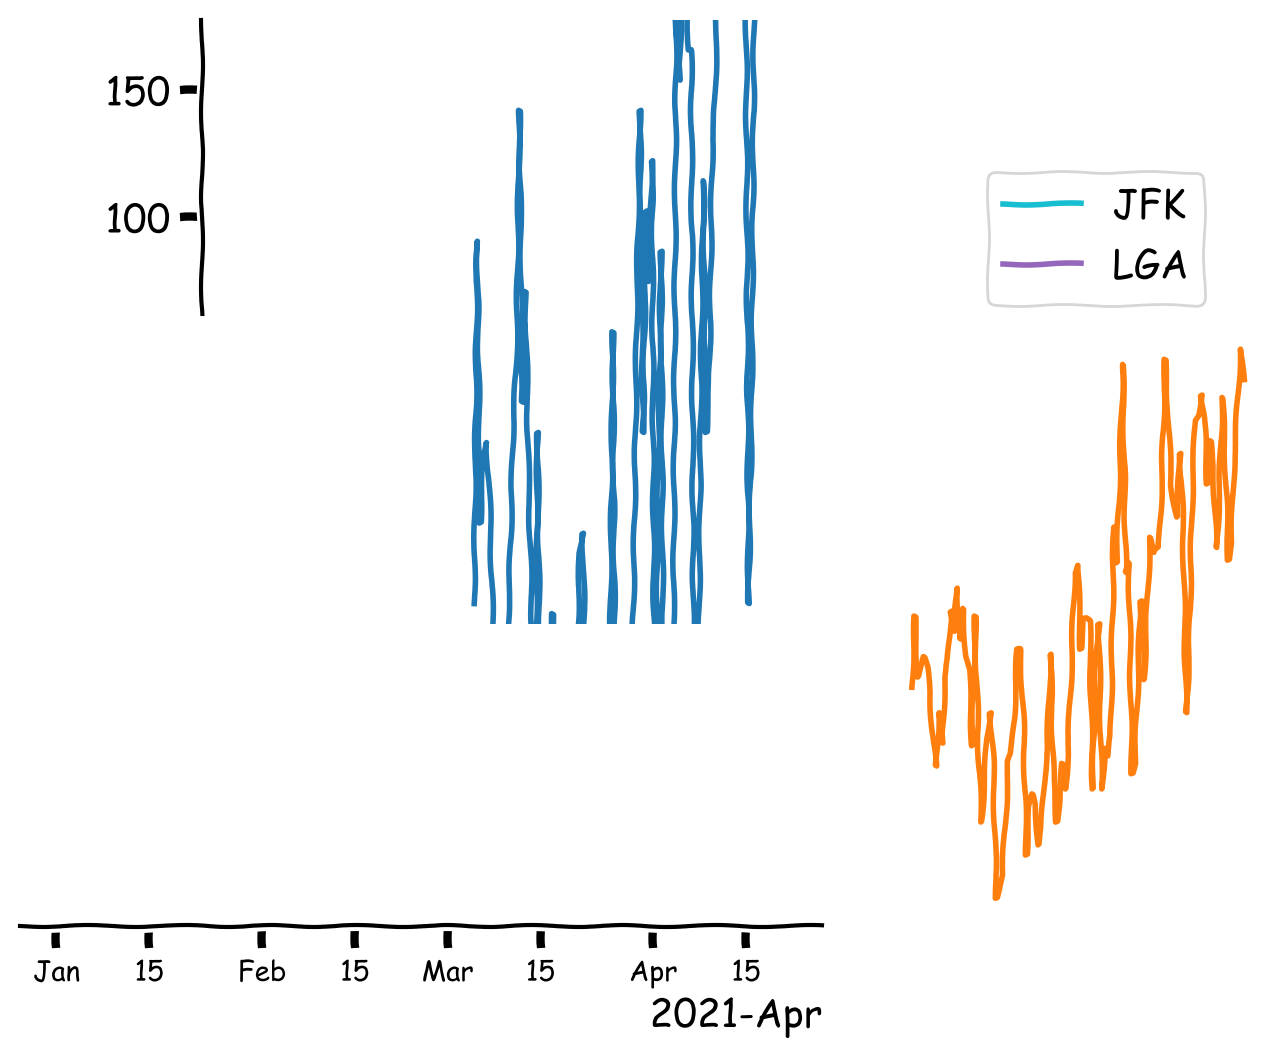
\includegraphics[width=.4\columnwidth]{exploding_artist.png}%
\label{fig:artist:union:glue}}
%\hfil
\subfloat[$\oplus$]{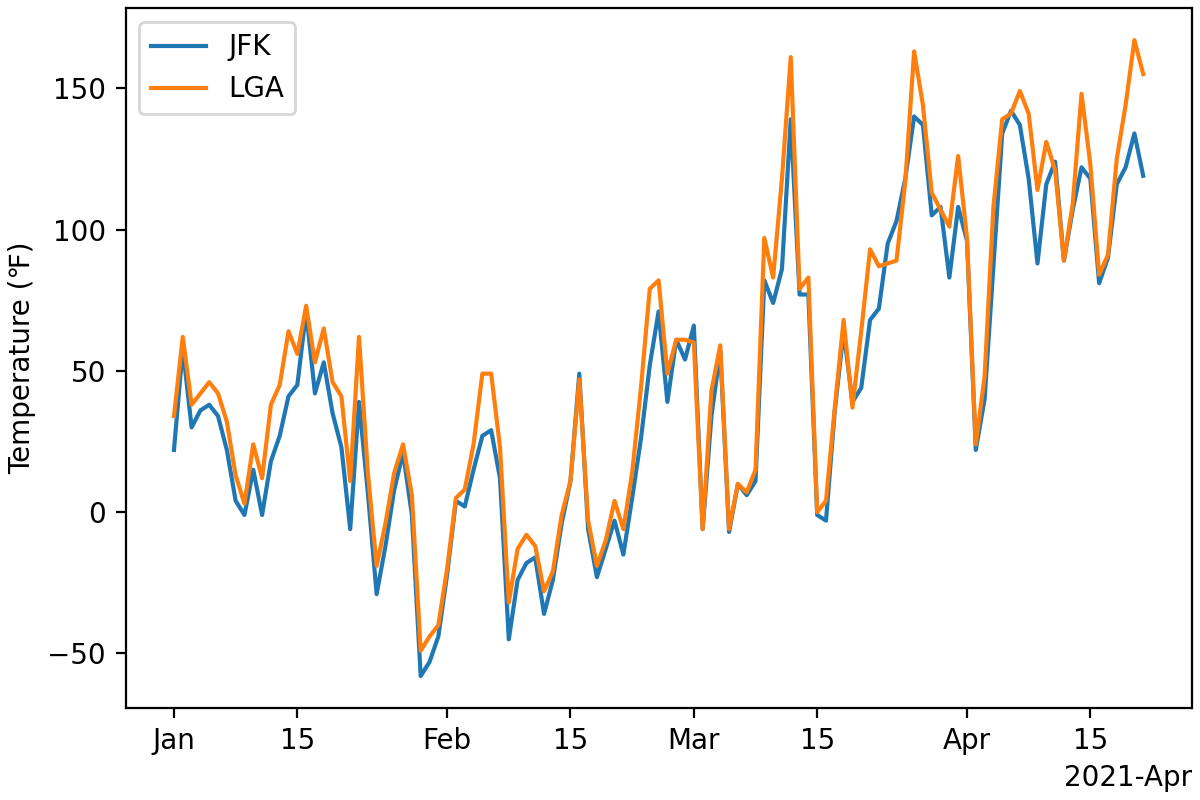
\includegraphics[width=.4\columnwidth]{combined_artist.png}%
\label{fig:artist:union:continuity}}
\caption{In \autoref{fig:artist:union:glue}, the outputs of various artist are independently rendered to the same graphic space. The inputs to the artists in \autoref{fig:artist:union:continuity} are sections over the same fiber bundle base space \dbase; therefore, they should share transformation functions to produce a consistent image. \note{add a border/make the same size/etc so 1 doesn't run over into two}}
\end{figure}

\note{is about building artist that preserves constraint A1 out of A2 + A3}
% generalizing sheaf to collection of sheafs w/ inclusion maps so can tell you how to assemble A1 + A2 such that that push out is preserved 
% when we build an artist out of nus and qs, this is how to preserve this 
% if the artist is a black box, what are the pre and post conditionsg
Visualizations generally consist of more than one visual element, for example line plots, a legend, axis ticks, spines, and labels. Many times, visualizations are generated from subsets of a larger data set, such as when using multiple views \cite{alboRadarComparativeEvaluation2016a} and brush-linked views \cite{beckerBrushingScatterplots1987,bujaInteractiveData1991}, and there is an expectation of consistency in how this data is visualized\cite{hullmanKeeping2018}. In \autoref{fig:artist:union:glue}, the disjointedness of the graphic lends itself to an interpretation that the data is disjoint, whereas the consistency of the visual encodings in \autoref{fig:artist:union:continuity} indicates that visual elements share data attributes. In this section, we describe how to express the structure of the data input in terms of  whether the sheaf objects $\sheaf_{\mathcal{\dtotal}}$ are disjoint or share attributes. We then propose that a topologically equivariant artist will preserve this structure in its output. 

\subsection{Union of Base Spaces}
\begin{figure}[h!]
  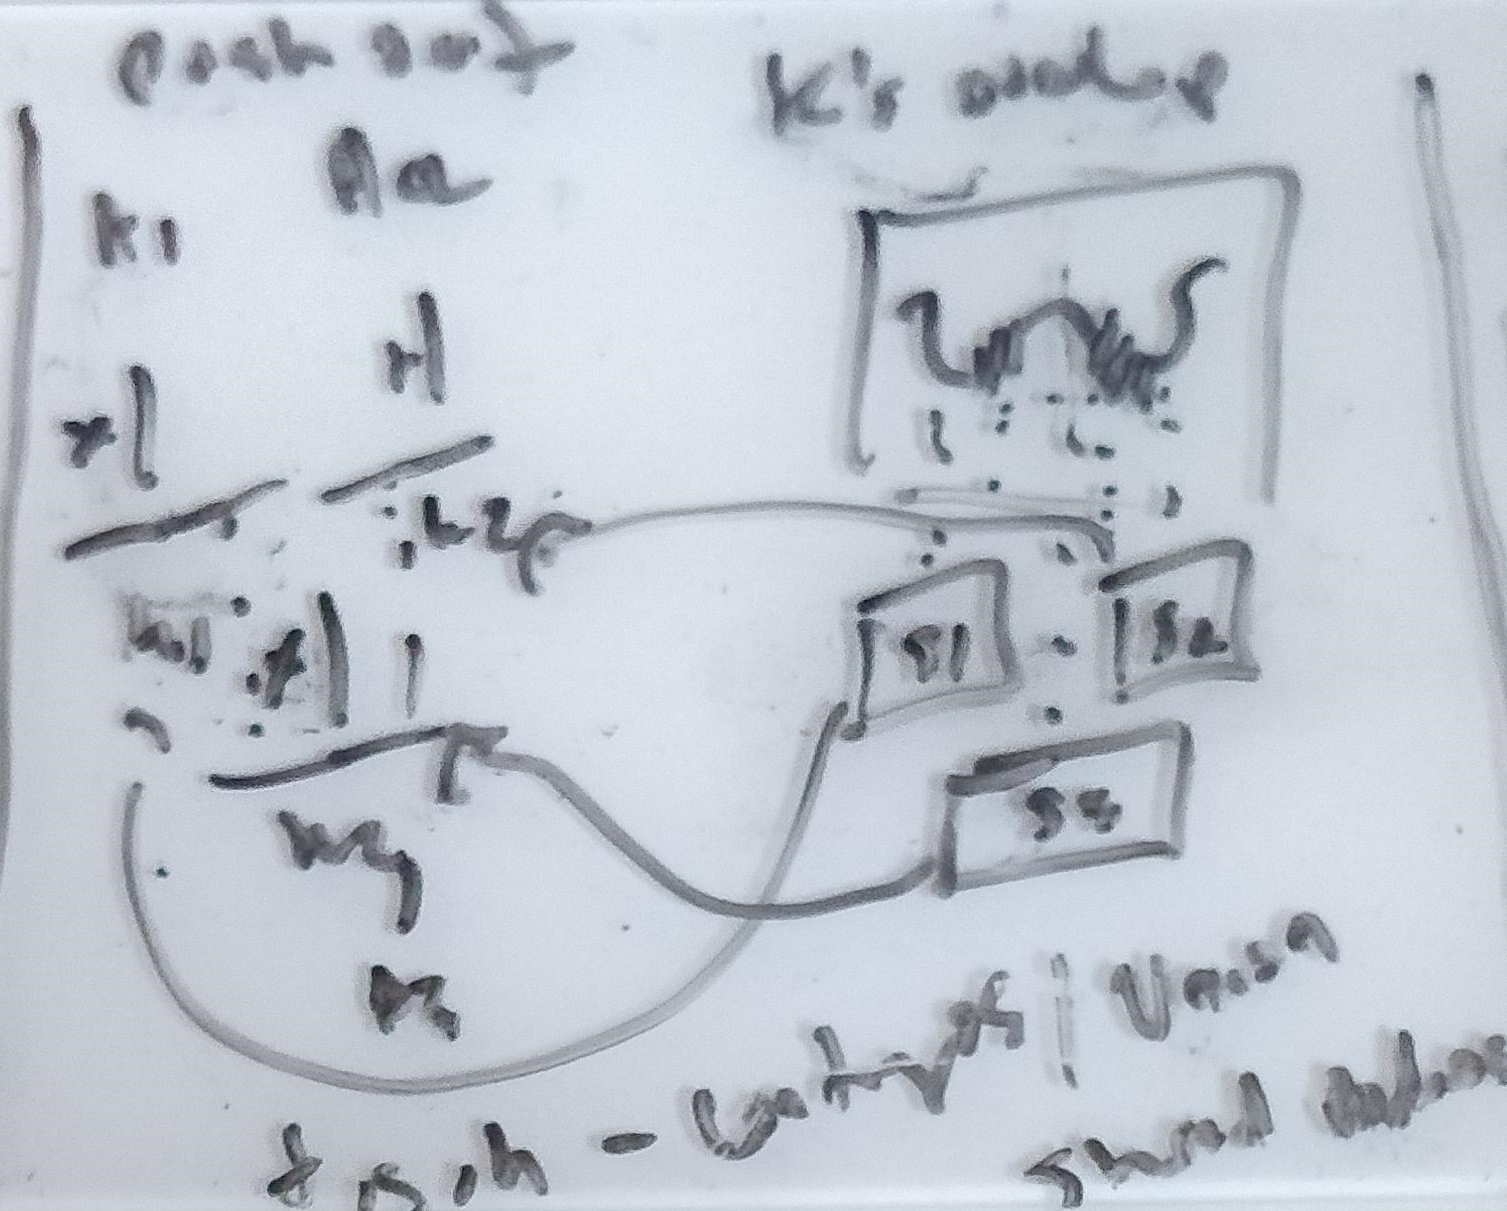
\includegraphics[width=\columnwidth]{union_k.png}
  \caption{}
  \label{fig:artist:compose:union_base}
\end{figure}

\begin{figure}[h!]
  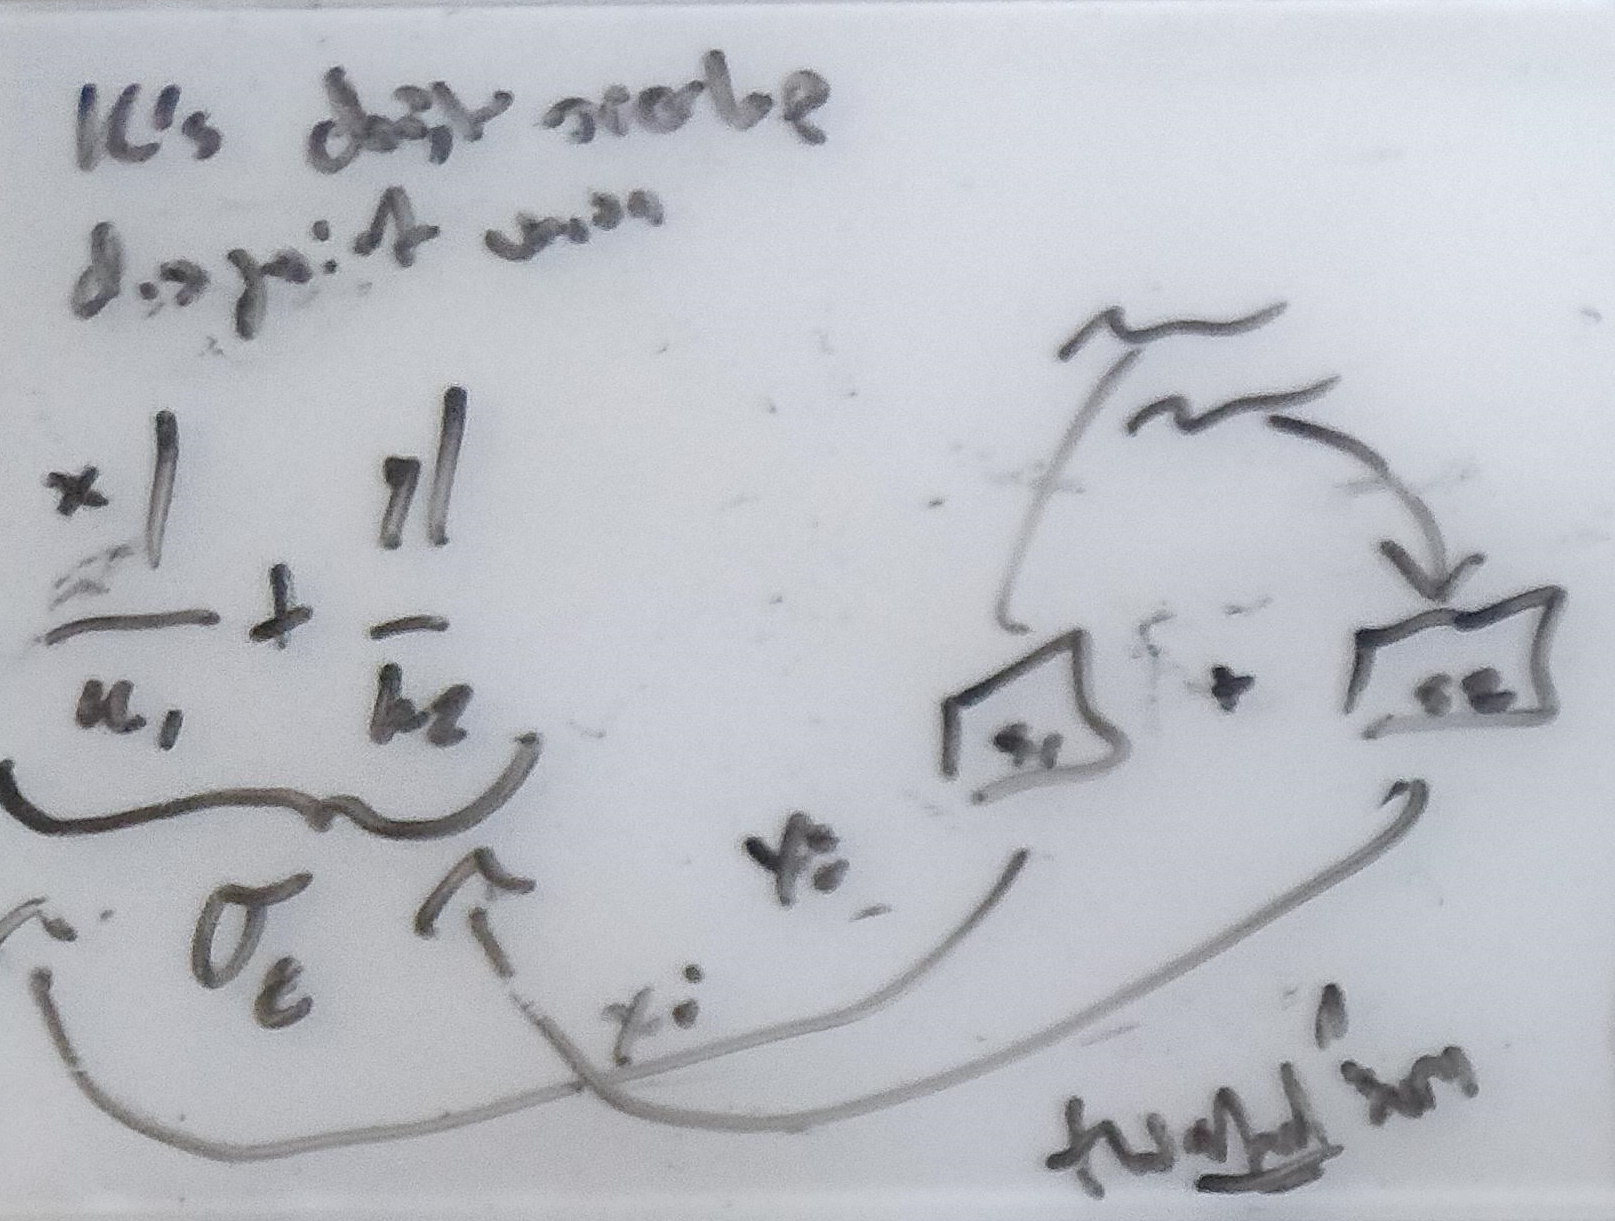
\includegraphics[width=\columnwidth]{disjoint_k.png}
  \caption{}
  \label{fig:artist:compose:disjoint_base}
\end{figure}

\begin{tikzcd}
  \dbase_{k} \arrow[d, "\iota", hook] \arrow[r, "\iota", hook] & \dbase_{j} \arrow[d, "i_{\dbase_j}"]      \\
  \dbase_{i} \arrow[r, "i_{\dbase_i}"]                         & \dbase_{i} \bigcup_{\dbase_{k}}\dbase_{j}
  \end{tikzcd}
where the functions $i_{\dbase_i},i_{\dbase_j}$ project  

\paragraph{Shared fibers}

\begin{figure}[h!]
  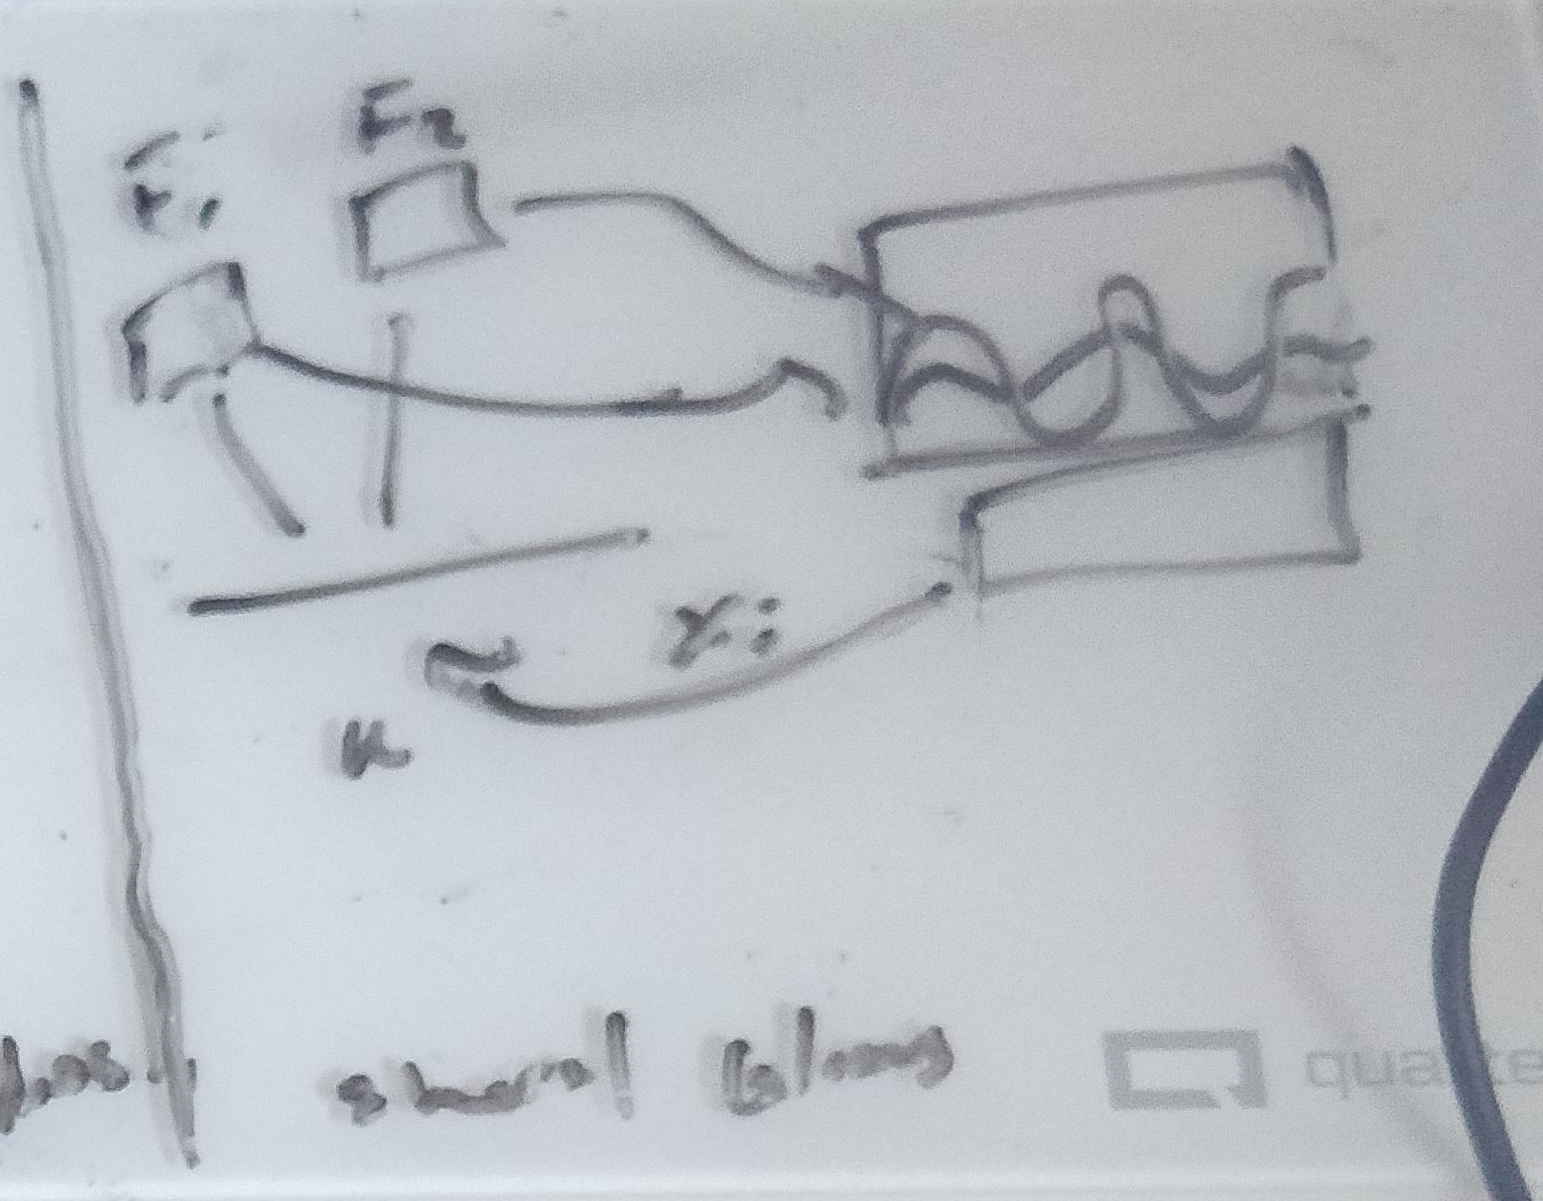
\includegraphics[width=\columnwidth]{intersection_f.png}
  \caption{}
  \label{fig:artist:compose:union_fiber}
\end{figure}


\section{Construction and formal properties of Artists}
\label{sec:artist:construction}
\begin{figure*}[h!]
  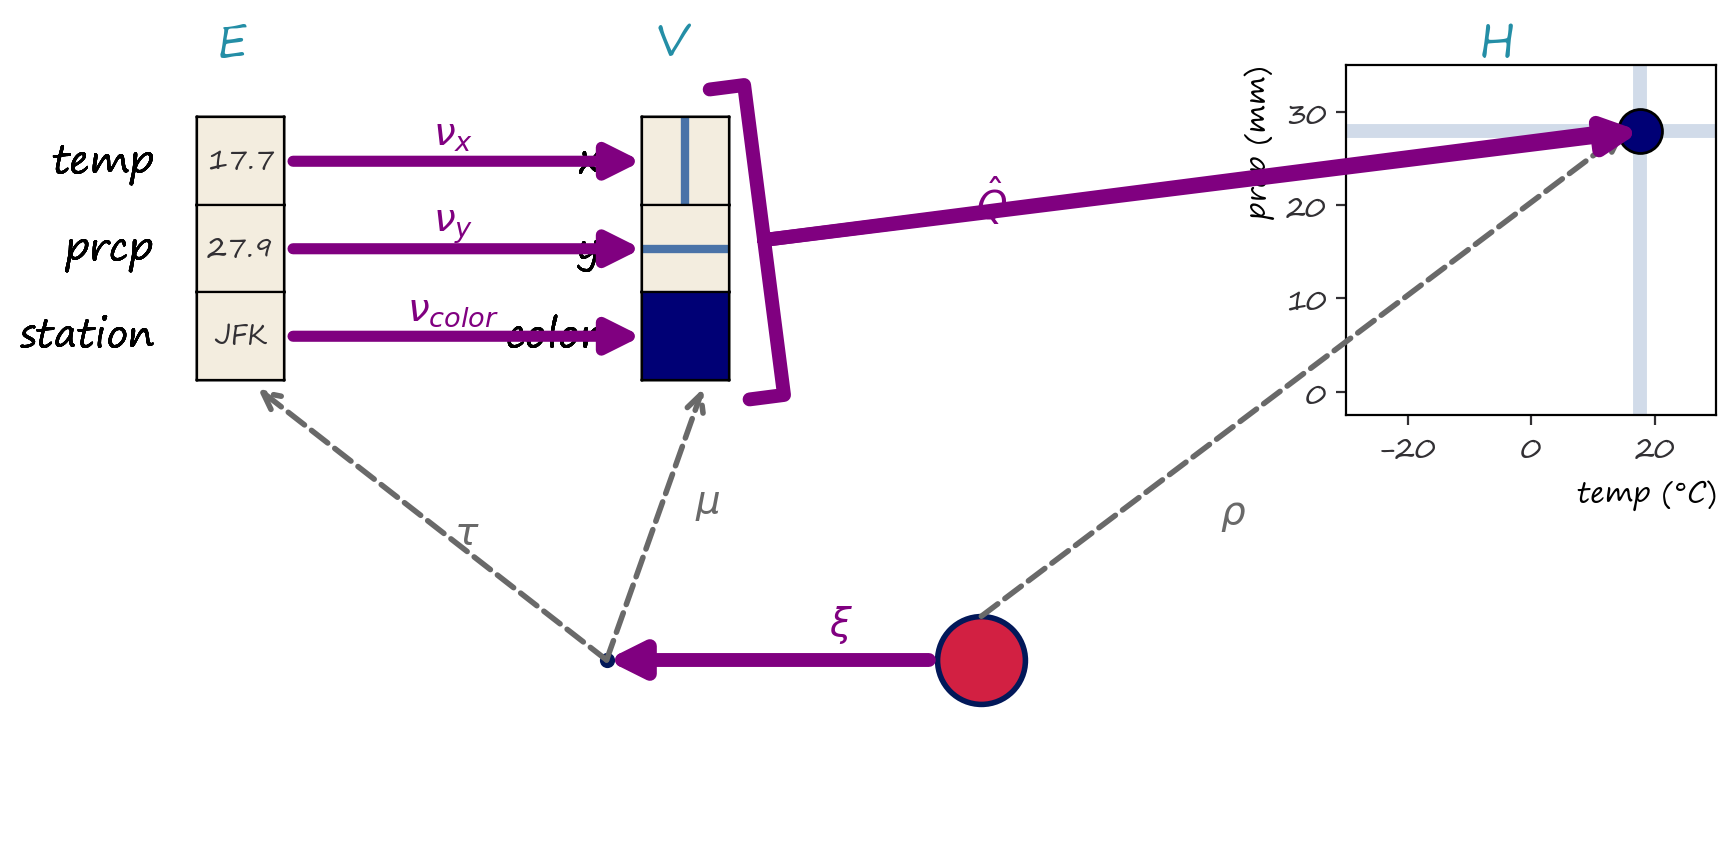
\includegraphics[width=\linewidth]{q.png}
  \caption{}
  \label{fig:constraints:q-overall}
\end{figure*}


\begin{definition} Following from \label{def:artist:} the artist \vartist is a special case of  natural transformations
  \begin{equation}
    \vartist: \Gamma(\dtotal, \dbase)\nrightarrow \Gamma(\gtotal, \gbase)
  \end{equation}
  between the profunctor objects $\Gamma(E),\Gamma(H)$ that preserves continuity and equivariance.
\end{definition}
  Natural transformations are functions that map functions between categories (functors) to other functors in a structure preserving way \cite{riehlCategoryTheoryContext, spanier1989algebraic, fongInvitationAppliedCategory2019}.

\begin{definition} We define the natural transformation \textcolor{artist}{Artist}  \vartist\ as the tuple $(\vindex, \vchannel, \vmark, \mathcal{\dtotal},\mathcal{\vtotal}, \mathcal{\gtotal})$ where
  \begin{enumerate}
    \item \vindex\ is a continuity preserving functor
    \item \vchannel\ and \vmark\ are equivariance preserving functors
    \item $\mathcal{\dtotal}$, $\mathcal{\vtotal}$, and $\mathcal{\gtotal}$ are profunctor categories of sheafs
    \item 
  \end{enumerate}
\end{definition}

\begin{equation}
  \label{eq:math:artist:diagram}
  \begin{tikzcd}
      \dtotal \arrow[r, "\vchannel"] \arrow[rd, "\pi"'] & \vtotal \arrow[d, "\pi"] & \vindex^*\vtotal \arrow[r, "\vmark"] \arrow[d, "\vindex^*\pi"'] \arrow[l, "\vindex^*"'] & \gtotal \arrow[ld, "\pi"] \\
                                            & \dbase                  & \gbase \arrow[l, "\vindex"']                                              &                    
      \end{tikzcd}
\end{equation}

\subsection{Data}
We model data as sections of a fiber bundle $(\dtotal, \pi, \dbase, \dfiber)$. We encode the continuity of the data as the \textcolor{base}{base space} $\dbase$. \note{does this go in intro?} The \textcolor{fiber}{fiber space} \dfiber\ is the space of all possible values of the data \autoref{eq:related-work:fiber}. We model the data as the section \dsection because, as described in \autoref{sec:related-work:fiber-bundles}, the section is the map from the indexing space \dbase to the space of possible data values \dfiber. Spivak's notation, as discussed in \autoref{sec:related-work:equivariance}, also allows for associating elements in a section with the field it comes from. This allows for field based selection of values, while inclusion allows for continuity (index) based selections. 


\begin{figure}[h!]
  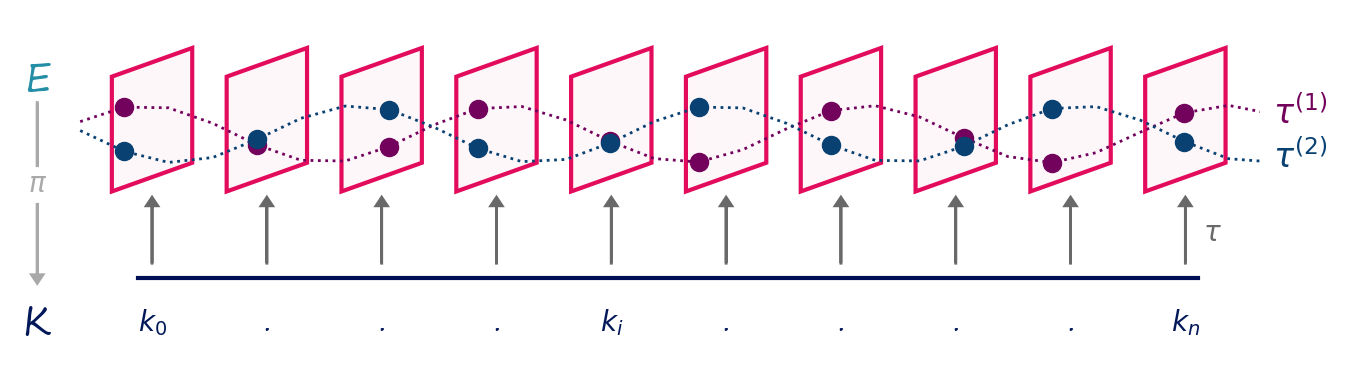
\includegraphics[width=\columnwidth]{fiberbundle.png}
  \caption{\note{replace with more concrete}}
  \label{fig:artist:data}
\end{figure}

One example of encoding data as a section of a fiber bundle is illustrated in \autoref{fig:artist:data}. In this example, the data is a \note{not totally decided yet} table of weather station data. Here we are interested in the time series of temperature values in the data, so we encode the continuity as the 1D interval \dbase. In this multivariate data set, the fields we want to visualize are \texttt{time}, \texttt{temperature}, and \texttt{station}. The fiber space \dfiber\ is the cartesian cross product of the fibers of each field
\begin{equation*}
  \dfiber = \dfiber_{time} \times \dfiber_{temperature} \times \dfiber_{station}
\end{equation*}
where each field fiber is the set of values that are valid for the field: 
\begin{align*}
  \dfiber_{time} &= \mathbb{R} \\
  \dfiber_{temperature} &= \mathbb{R}\\
  \dfiber_{station} &= \{s_0, s_1, \cdots, s_i, \cdots, s_n\} 
\end{align*}

The section \dsection\ is the abstraction of the data being visualized. The section at a point $k \in K$ in the base space returns a value from each field in the fiber.
\begin{equation*}
  \tau(k) = ((time, t_k); (precipitation, p_k); (station\;name, n_k))
\end{equation*}


\subsection{Graphic} 
The object of the graphic category $\mathcal{\gtotal}$ is the fiberbundle \gtotal. The bundle \gtotal\ has the same structure as the data bundle \dtotal

\begin{equation}
  \begin{tikzcd}[ampersand replacement=\&]
      \gfiber \arrow[r, hook] \& \gtotal \arrow[d, "\pi"'] \\
                        \& \gbase \arrow[u, "\gsection"', bend right]
  \end{tikzcd}
\end{equation}
with a fiber space \gfiber\ embedded in the total space \gtotal\ and a section map $\gsection:\gbase\rightarrow\gtotal$. The attributes of the graphic bundle $(\gtotal, \pi, \gfiber, \gbase)$ encode attributes of the graphic and display space 

\begin{LaTeXdescription}
\item [\textcolor{base}{base space} \gbase] continuity of display space (e.g. screen, 3D print)
\item [\textcolor{fiber}{fiber space} \gfiber] attributes of the display space (e.g a pixel = (x,y,r,g,b,a))
\item [\textcolor{section}{section} \gsection] graphic generating function
\end{LaTeXdescription}.

We represent the graphic output as a fiber bundle because it is an abstraction that is generalizable to various output mediums (screens, 3D prints) and types of graphics. In this work, \gtotal\ assumes the the display is an idealized 2D screen and \gsection\ is an abstraction of rendering. For example, \gsection\ can be a specification such as PDF\cite{bienz1993portable}, SVG\cite{quintScalable2003} or an OpenGL scene graph\cite{CarsonOpenGL1997}, or a rendering engine such as Cairo\cite{CairographicsOrg} or AGG\cite{shemanarevAntiGrainGeometry}.

\begin{figure}[h!]
  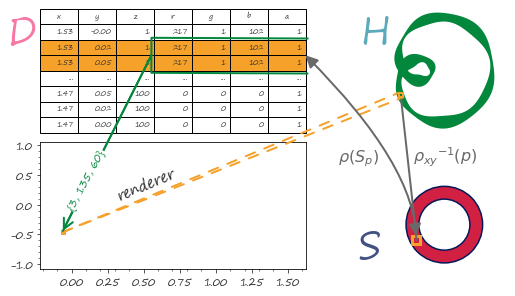
\includegraphics[width=\columnwidth]{render.png}
  \caption{}
  \label{fig:artist:graphic}
\end{figure}

\begin{example}
As illustrated in \autoref{fig:artist:graphic}, 
\end{example}

\subsection{Visualization Library Components}
\subsubsection{Graphic to Data: \vindex}
\begin{equation}
  \begin{tikzcd}
      \dtotal \arrow[d, "\pi"'] & \gtotal \arrow[d, "\pi"'] \\
      \dbase                   & \gbase \arrow[l, "\vindex"']
  \end{tikzcd}
  \label{eq:math:graphic:vindex}
\end{equation}

The functor $\vindex$ is a deformation retract, which means....\cite{hatcherAlgebraicTopology2002,spanier1989algebraic}

\subsubsection{Visual Bundle \vtotal}
\begin{equation}
  \begin{tikzcd}[ampersand replacement=\&]
      \vfiber \arrow[r, hook] \& \vtotal \arrow[d, "\pi"'] \\
                        \& \dbase \arrow[u, "\vsection"', bend right]
  \end{tikzcd}
\end{equation}

\subsubsection{Data to Visual Encodings: \vchannel} %look at what K&S call these stages
Visual encoding functions \vindex\ are functors because they are expected to preserve structure on the data and visual side, as discussed in \autoref{sec:related-work:equivariance}. 

 This constraint is expressed in our construction of \vchannel


\begin{figure}[!h]
  \centering
  \subfloat[Artists with shared $\mu_i$ renderered correctly]{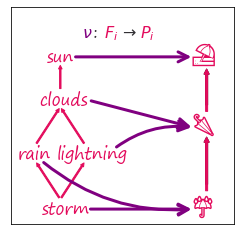
\includegraphics[width=1.2in]{partial_fixed.png}%
  \label{fig_first_case}}
  %\hfil
  \subfloat[Artists without shared $\mu_i$]{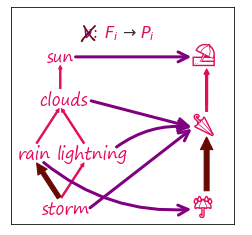
\includegraphics[width=1.2in]{partial_invalid.png}%
  \label{fig_second_case}}
  \caption{Simulation results for the network.}
  \label{fig_sim}
  \end{figure}

\begin{equation}
  \label{eq:math:artist:nu}
  \{\vchannel_{0}, \ldots, \vchannel_{n}\}: \{\dsection_{0}, \ldots, \dsection_{n}\} \mapsto \{\vsection_{0}, \ldots, \vsection_{n}\}
\end{equation}

We enforce the equivariance constraint

\begin{equation}
  \label{eq:math:artist:nu_commute}
\begin{tikzcd}
  \dtotal_i \arrow[r] \arrow[r, "\vchannel_i"] \arrow[d, "m_{\delement}"'] & \vtotal_i \arrow[d, "m_{\velement}"] \\
  \dtotal_i \arrow[r, "\vchannel_i"]                           & \vtotal_i               
\end{tikzcd}
\end{equation}

One advantage of expressing the data to visual encoding $\vchannel_i$ as a functor from data fiber $\dfiber_i$ to $\vfiber_i$ is that it lets us formally express that encodings are bound to data and therefore should be consistent across views, as proposed by Hullamn and Qu\cite{hullmanKeeping2018}.

\subsubsection{Visual to Graphic: \vmark} % look at what K&S call these stages
Visual encodings to something like marks 
\begin{figure}[!h]
  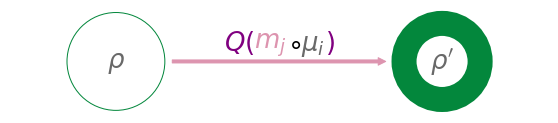
\includegraphics[width=\columnwidth]{diff_type_q.png}
  \caption{rework this as a commutative box w/ the r in E row associated w/ this qhat(k)}
\end{figure}
 
\section{Case Study}
\label{sec:case-study}
\begin{figure}[h!]
  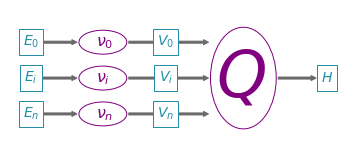
\includegraphics[width=\columnwidth]{path_of_q.png}
    \caption{\note{add in xi!}}
  \label{fig:api}
\end{figure}
We implement the \textbf{arrows} in \autoref{fig:api}. \mintinline{python}{axesArtist} is a parent artist that acts as a screen. This allows for the composition described in                                           \autoref{sec:artist:union}

\subsection{\vartist}
\begin{minted}{python}
for local_tau in axesArtist.artist.data.query(screen_bounds, dpi):
    mu = axesArtist.artist.graphic.mu(local_tau)
    rho = axesArtist.artist.graphic.qhat(**mu)
    H = rho(renderer)
\end{minted}

where the artist is already parameterized with the \vindex\ functions and which fibers they are associated to:

\begin{minted}{python}
\end{minted}


\subsubsection{\vindex}
\subsubsection{\vchannel}
\subsubsection{\vmarkd}



\section{Discussion}
\subsection{Limitations}
\subsection{future work}

\section{Conclusion}
The conclusion goes here.


\appendices
\section{Rendering: \gsection}
\section{Manufacturing $\vmarkd \leftarrow \vmark$}
\begin{equation}
  \begin{tikzcd}
      \textcolor{gray!50}{\dtotal} \arrow[r, "\vchannel", color=gray!50] \arrow[rd, "\pi"', color=gray!50] & \vtotal \arrow[d, "\pi"']                  & \vindex^*\vtotal \arrow[r, "\vmark", color=gray!50] \arrow[d, "\vindex^*\pi"'] \arrow[l,  "\vindex^*"'] & \textcolor{gray!50}{\gtotal} \arrow[ld, "\pi", color=gray!50] \\ & \dbase \arrow[u, "\vsection"', bend right] & \gbase \arrow[l, "\vindex"'] \arrow[u, "\vindex^*\vsection"', bend right]               &                          
      \end{tikzcd}
      \label{eq:math:artist:qhat}
\end{equation}



% use section* for acknowledgment
\ifCLASSOPTIONcompsoc
  % The Computer Society usually uses the plural form
  \section*{Acknowledgments}
\else
  % regular IEEE prefers the singular form
  \section*{Acknowledgment}
\fi


The authors would like to thank...


% Can use something like this to put references on a page
% by themselves when using endfloat and the captionsoff option.
\ifCLASSOPTIONcaptionsoff
  \newpage
\fi

% trigger a \newpage just before the given reference
% number - used to balance the columns on the last page
% adjust value as needed - may need to be readjusted if
% the document is modified later
%\IEEEtriggeratref{8}
% The "triggered" command can be changed if desired:
%\IEEEtriggercmd{\enlargethispage{-5in}}

% references section

% can use a bibliography generated by BibTeX as a .bbl file
% BibTeX documentation can be easily obtained at:
% http://mirror.ctan.org/biblio/bibtex/contrib/doc/
% The IEEEtran BibTeX style support page is at:
% http://www.michaelshell.org/tex/ieeetran/bibtex/
\bibliographystyle{IEEEtran}
% argument is your BibTeX string definitions and bibliography database(s)
\bibliography{bibliography}

% biography section 
% If you have an EPS/PDF photo (graphicx package needed) extra braces are
% needed around the contents of the optional argument to biography to prevent
% the LaTeX parser from getting confused when it sees the complicated
% \includegraphics command within an optional argument. (You could create
% your own custom macro containing the \includegraphics command to make things
% simpler here.)
%\begin{IEEEbiography}[{\includegraphics[width=1in,height=1.25in,clip,keepaspectratio]{mshell}}]{Michael Shell}
% or if you just want to reserve a space for a photo:

%\begin{IEEEbiography}{Michael Shell}
%\end{IEEEbiography}

% if you will not have a photo at all:
\begin{IEEEbiographynophoto}{Hannah Aizenman}
Biography text here.
\end{IEEEbiographynophoto}

\begin{IEEEbiographynophoto}{Thomas Caswell}
  Biography text here.
\end{IEEEbiographynophoto}
% insert where needed to balance the two columns on the last page with
% biographies
%\newpage

\begin{IEEEbiographynophoto}{Michael Grossberg}
Biography text here.
\end{IEEEbiographynophoto}

% You can push biographies down or up by placing
% a \vfill before or after them. The appropriate
% use of \vfill depends on what kind of text is
% on the last page and whether or not the columns
% are being equalized.

%\vfill

% Can be used to pull up biographies so that the bottom of the last one
% is flush with the other column.
%\enlargethispage{-5in}

% that's all folks
\end{document}


